\documentclass[11pt]{article}

% ====================================================================
%  Calibrated Joint Uncertainty Across Scales for Small-Area Estimation:
%  A Bayesian Model-Based Geostatistics Framework with a Semi-Dense
%  Coarse-Layer Tree Prior  (BARTSIMP-PG-SD)
%  Target venue: JASA Applications & Case Studies / AOAS
% ====================================================================

\usepackage[margin=1in]{geometry}
\usepackage{amsmath,amssymb,amsthm}
\usepackage{bm}
\usepackage{graphicx}
\usepackage{booktabs}
\usepackage{multirow}
\usepackage{array}
\usepackage[round]{natbib}
\usepackage{microtype}
\usepackage{hyperref}
\usepackage{xcolor}
\usepackage{enumitem}

\hypersetup{colorlinks=true, linkcolor=blue!55!black, citecolor=blue!55!black,
            urlcolor=blue!55!black}

% ---- theorem environments ----
\newtheorem{theorem}{Theorem}
\newtheorem{proposition}{Proposition}
\newtheorem{lemma}{Lemma}
\newtheorem{assumption}{Assumption}
\theoremstyle{remark}
\newtheorem{remark}{Remark}

% ---- status macros for honest theory labels ----
\newcommand{\PROVEN}{\textnormal{\textbf{\textcolor{green!45!black}{[PROVEN]}}}}
\newcommand{\CONJ}{\textnormal{\textbf{\textcolor{orange!75!black}{[CONJECTURED]}}}}
\newcommand{\PROVENMOD}{\textnormal{\textbf{\textcolor{green!40!black}{[PROVEN, modulo stated fixes]}}}}

% ---- notation macros ----
\newcommand{\R}{\mathbb{R}}
\newcommand{\E}{\mathbb{E}}
\newcommand{\Var}{\mathrm{Var}}
\newcommand{\N}{\mathrm{N}}
\newcommand{\logit}{\operatorname{logit}}
\newcommand{\PG}{\mathrm{PG}}
\newcommand{\dz}{d_0}
\newcommand{\chia}{\chi^a}
\newcommand{\Vsmp}{V^a_{\mathrm{smp}}}
\newcommand{\bartsimp}{\textsc{bartsimp-pg}}
\newcommand{\bartsimpsd}{\textsc{bartsimp-pg-sd}}
\newcommand{\cov}{\mathrm{cov}}
\newcommand{\ratio}{\mathrm{RMSE}/\overline{\mathrm{sd}}}

\title{\bf Calibrated Joint Uncertainty Across Scales for Small-Area
Estimation: A Bayesian Model-Based Geostatistics Framework with a
Semi-Dense Coarse-Layer Tree Prior}

\author{[Author block omitted for review]}
\date{}

\begin{document}
\maketitle

% ====================================================================
\begin{abstract}
% ====================================================================
Small-area estimation (SAE) from complex survey data must carry honest
uncertainty from the point/cluster scale at which modeling occurs to the
area scale at which policy decisions are made. We present a Bayesian
model-based-geostatistics (MBG) framework that couples a Bayesian additive
regression tree (BART) mean, a structured SPDE--Mat\'ern Gaussian-process (GP)
spatial field, and P\'olya--Gamma augmentation for the binomial-logit
likelihood, and that produces genuine \emph{joint} posterior draws of the
latent prevalence surface. From these draws, credible intervals for any
area-average functional are obtained by aggregation, so the same fitted model
delivers uncertainty quantification (UQ) at the pixel, cluster, and
administrative-area scales simultaneously. Across a ten-method benchmark, this
framework is the only one whose calibration ratio (root-mean-square error over
posterior standard deviation) stays near one at \emph{every} aggregation scale;
the competitors are each calibrated at only a single crossing scale. The framework
has one residual soft spot: the area (Admin-1) coverage sits modestly below
nominal because the flexible tree mean carries a slowly-vanishing
low-frequency (``non-Donsker'') bias that survives aggregation. We diagnose this
as a \emph{center} bias---not a width problem---and remedy it with a
\emph{semi-dense coarse-layer tree prior}: a hard depth-floor $\dz \approx
\sqrt{\log N}$ that forces the coarsest tree layers to remain dense, after
\citet{castillo2021cart}. The depth-floor is a single prior knob (three
localized edits, essentially zero added compute) that is \emph{exactly} the
hypothesis our target forward-route functional Bernstein--von Mises (BvM)
theorem requires. In a paired, matched-seed simulation study the floor recenters
Admin-1 80\% coverage toward nominal across a broad plateau of $\dz \ge 1$
($0.79 \to 0.815$--$0.827$) and across aggregation scales and spatial amplitudes,
\emph{without} disturbing the near-nominal pixel/cluster/95\% calibration. We are
deliberate about the strength of evidence: the primary paired contrast is
right-signed but modest ($\Delta\cov_{80}=+0.014\pm0.010$ at 24 replicates, below
two Monte-Carlo standard errors), and the corroborating sensitivity, scale, and
adversarial sweeps---not the single primary contrast---carry the claim. On the
theory side we state a Mat\'ern-only Admin-1 functional BvM (\PROVEN, modulo a
re-regime fix) and a single-tree Gaussian combined BvM (\CONJ, no fatal holes),
and we are explicit that the binomial-logit transfer and the deployed-dimension
($p\approx 49$) regime remain open.
\end{abstract}

\noindent\textbf{Keywords:} small-area estimation; model-based geostatistics;
Bayesian additive regression trees; P\'olya--Gamma; Mat\'ern/SPDE; functional
Bernstein--von Mises; calibrated uncertainty; survey statistics.

% ====================================================================
\section{Introduction}\label{sec:intro}
% ====================================================================

National health and development programs are increasingly governed by
\emph{small-area} statistics: the prevalence of child wasting in an
administrative district, the under-five mortality rate in a sub-county, the
coverage of an intervention in a province. These quantities are estimated from
complex household surveys---most prominently the Demographic and Health Surveys
\citep[DHS;][]{dhs2014kenya}---that are designed to be representative at coarse
scales but are sparse,
clustered, and stratified at fine scales. The statistical challenge is a
\emph{scale mismatch}: the policy deliverable is an area-level average, but the
data and the natural model live at the point/cluster level. A credible method
must therefore carry honest uncertainty \emph{through aggregation}, from the
clusters where measurements are taken to whatever administrative partition a
decision-maker cares about, and must do so when the covariate--response
relationship is nonlinear and there is residual spatial structure the covariates
do not explain.

\paragraph{Two cultures, each calibrated at one scale.}
Existing methodology splits into two cultures, and---this is the gap we
target---each is calibrated at only one aggregation scale. The
\emph{design-based} culture (direct/H\'ajek estimators, model-assisted
generalized regression, and the more recent prediction-powered inference of
\citealp{angelopoulos2023ppi}) is correct where its independent-residual variance
model holds, but it supplies no pixel- or cluster-level uncertainty and
understates standard errors under design effects. The \emph{model-based
geostatistics} (MBG) culture \citep{diggle1998mbg,rue2009inla,lindgren2011spde}
places a latent Gaussian field over space and aggregates it to areas; the INLA
SPDE--Mat\'ern model is the standard in low- and middle-income-country (LMIC)
disease mapping, and disaggregation regression \citep{nandi2023disaggregation}
is its native binomial, joint-UQ analogue. Both rest on a \emph{linear} mean.
Where the true mean is curved or interacting, that linear mean misfits, and the
misfit surfaces as a \emph{scale-dependent} coverage error: calibrated at the
coarse crossing scale, miscalibrated elsewhere. Flexible-mean machine learning
enters from two directions but does not close the gap. Bayesian additive
regression trees \citep[BART;][]{chipman2010bart} give a well-calibrated
\emph{pointwise} nonparametric mean, but with no spatial term they collapse at
the area functional (we measure Admin-1 80\% coverage of $0.29$ for vanilla
BART). Spatial random forests \citep[RF-GLS;][]{saha2023rfgls} and related
spatial-ML methods restore a spatial mean, but emit only \emph{marginal}
per-cluster intervals and reach nominal coverage through a constant bias or a
laundered interval width that holds at one scale and fails at another. None of
these delivers a coherent \emph{joint} area-mean law that is calibrated across
scales.

\paragraph{Contribution.}
We make the calibrated-joint-UQ-across-scales property the headline and deliver
it with a framework---\bartsimpsd---built from three known ingredients and one
new prior knob. The mean is a BART ensemble; the spatial field is an
SPDE--Mat\'ern GP \citep{lindgren2011spde}; the binomial-logit likelihood is
handled by P\'olya--Gamma augmentation \citep{polson2013polyagamma}, which renders
the model conditionally Gaussian and lets us draw the latent surface
\emph{jointly} across all clusters. From those joint draws, the posterior of any
bounded linear functional of the surface---in particular the area-average
prevalence---follows by aggregation, carrying the full cross-cluster covariance
that marginal-interval competitors lack. On a ten-method benchmark this framework
is the unique method whose calibration ratio stays near one at every aggregation
scale (Section~\ref{sec:results}).

The framework has one residual soft spot, and identifying and fixing it is the
specific methodological novelty. The Admin-1 coverage sits modestly \emph{below}
nominal ($\cov_{80}\approx 0.77$ versus $0.80$) while the 95\% coverage is
near-nominal and the calibration ratio is only slightly above one (validation
ratio $\approx 1.034$; production-surface ratio $\approx 1.08$). Because the
ratio exceeds one only slightly while the lower quantile lags, the deficit is a
\emph{center} bias, not a width problem: a standardized bias of $\delta =
\sqrt{\mathrm{ratio}^2-1}$, i.e.\ $\delta\approx 0.26$ at the validation ratio
and $\delta\approx 0.4$ posterior SD at the production-surface ratio
(Section~\ref{sec:estimand}). This is the predicted
\emph{non-Donsker} effect of the tree mean: the flexible mean carries a slowly
vanishing low-frequency bias that the credible band cannot see, and that
survives area-averaging precisely because the area mean loads on the coarse,
low-resolution component of the surface---the very component a pruning tree prior
under-represents. \citet{castillo2021cart} prove, in a single-tree Gaussian
setting, that tree-prior functional under-coverage is caused by the prior pruning
its coarse layers, and that the remedy is a \emph{prior modification}---keep the
coarse layers dense---rather than estimator-side debiasing. We deploy exactly this:
a \emph{semi-dense coarse-layer prior}, implemented as a hard depth-floor $\dz
\approx \sqrt{\log N}$ that forbids pruning of the coarsest $\dz$ tree layers. The
floor is a single Bayesian-coherent knob (three localized edits to the sampler,
essentially zero added compute) that recenters the Admin-1 posterior toward
nominal \emph{without} widening the fine-scale bands, and it is the same prior
object that our target functional-BvM theorem requires---a rare alignment of the
deployed method with the theory.

\paragraph{Honest framing of the evidence.}
We are explicit, throughout, about the strength of the evidence---a discipline a
top applications venue rewards. In the primary matched-seed paired comparison
(24 replicates), the floor moves Admin-1 $\cov_{80}$ from $0.762$ to $0.777$, a
paired $\Delta\cov_{80}=+0.0145\pm0.0102$, right-signed and accompanied by a
paired bias reduction at two Monte-Carlo standard errors, but itself below two
Monte-Carlo standard errors and below a pre-registered $+0.02$ bar. The claim is
carried not by that single contrast but by the consistency of three
corroborating sweeps: a $\dz$ sensitivity sweep in which coverage rises to a
broad plateau ($0.79\to 0.815$--$0.827$ for all $\dz\ge1$) with the pixel and 95\%
guardrails flat; an aggregation-scale sweep in which the floored method is at
least as well-covered at every scale $A\in\{5,20,40\}$; and an adversarial
spatial-amplitude sweep in which the floor recenters coverage \emph{toward}
nominal from both sides. We likewise state up front the limitations we do not
fix: the binomial-logit conservative-coverage theory remains conjectural (the
rigorous theorem is a Gaussian single-tree sibling), the clean theorem's
dimension condition $s_a > p/2$ fails at the deployed dimension $p\approx 49$,
and admin-level observation overdispersion (design effects) is an acknowledged
non-robust regime that the depth-floor, a mean-recentering knob, does not address.

\paragraph{Outline.}
Section~\ref{sec:related} positions the framework against the two cultures and
the prior-theoretic literature. Section~\ref{sec:methods} specifies the model,
the P\'olya--Gamma sampler, the semi-dense depth-floor, and the area functional.
Section~\ref{sec:theory} states the theoretical properties with explicit
honest status labels. Section~\ref{sec:results} reports the benchmark and the
three corroborating sweeps. Section~\ref{sec:discussion} discusses performance,
robustness, anomalies, limitations, and future work, and
Section~\ref{sec:conclusion} concludes. Supplementary tables are in the Web
Appendix.

% ====================================================================
\section{Related Work}\label{sec:related}
% ====================================================================

\paragraph{Design-based and model-assisted SAE.}
The reference treatment of small-area estimation is \citet{rao2015small}.
Direct estimators and model-assisted generalized regression are design-consistent
but provide no surface-level uncertainty and understate standard errors under
the clustering and stratification of survey designs; prediction-powered inference
\citep{angelopoulos2023ppi} sharpens area-level point estimates with auxiliary
predictions but, like the others, emits an area-direct interval with no pixel UQ.
These methods are the right tool when only an area mean is needed and the design
variance model holds; they are not aggregable to an arbitrary partition with a
coherent joint law, which is our requirement.

\paragraph{Linear-mean model-based geostatistics.}
The MBG tradition \citep{diggle1998mbg} models a latent Gaussian field and is
realized at scale through INLA \citep{rue2009inla} and the SPDE--Mat\'ern
representation \citep{lindgren2011spde}, which turns a continuously-indexed
Mat\'ern field into a sparse Gaussian Markov random field over a mesh. Areal
disease-mapping baselines---the intrinsic CAR model \citep{besag1991icar} and
binomial CAR/BYM regressions \citep{wakefield2007disease}---and disaggregation
regression \citep{nandi2023disaggregation}, which fits a binomial areal model
with joint TMB uncertainty, are the field-standard comparators. All carry a
\emph{linear} mean, so a curved or interacting truth induces a mean-misfit bias
that is averaged away only at the coarse scale; their calibration ratio sweeps
through one as the aggregation scale varies (the ``averageable-misfit camp'').

\paragraph{Flexible-mean and spatial machine learning.}
BART \citep{chipman2010bart} supplies a calibrated pointwise nonparametric mean
and is the mean model we adopt; \citet{jeong2023artofbart} establish its adaptive
minimax contraction rates in additive H\"older classes, and
\citet{petrillo2024bartgp} characterize its Gaussian-process limit. Without a
spatial term, however, BART has no field to aggregate and collapses at the area
functional. Spatial random forests \citep[RF-GLS;][]{saha2023rfgls} and vendored
CAR-forest variants (SPARforest) restore a spatial mean but produce only marginal
per-cluster Gaussian intervals; they reach nominal coverage by a constant bias or
a laundered width and are therefore calibrated at only one crossing scale (the
``constant-bias camp''). The two-camp framing---constant-bias methods calibrated
at the fine crossing, averageable-misfit methods at the coarse crossing---is the
rhetorical and empirical spine of our claim that no competitor holds calibration
at \emph{every} scale (Section~\ref{sec:results}).

\paragraph{Latent-variable augmentation.}
Conditional conjugacy for the binomial-logit model is restored by P\'olya--Gamma
augmentation \citep{polson2013polyagamma}; Albert--Chib probit
\citep{albert1993bayesian} and Holmes--Held logit \citep{holmes2006bayesian} are
the classical alternatives. The augmentation choice affects credible-interval
width but not the point estimate (a width-only knob we discuss in
Section~\ref{sec:discussion}); we adopt P\'olya--Gamma because it yields the
cleanest conditionally-Gaussian sampler for the joint surface.

\paragraph{Prior-theoretic basis: BvM and the semi-dense fix.}
The theory we build on is the functional Bernstein--von Mises program.
\citet{knapik2011bayesian} (hereafter KvdVvZ) give functional-BvM and coverage
results for Gaussian-process priors via a representer-decay condition; this is the
machinery for our Mat\'ern-only Admin-1 result (Theorem~\ref{thm:matern}).
\citet{castillo2021cart} prove---this is the linchpin---that tree-prior functional
under-coverage is a coarse-layer-\emph{pruning} phenomenon, remediable by a
\emph{semi-dense} prior that keeps the coarsest $\dz \asymp \sqrt{\log n}$ layers
dense, rather than by debiasing. We import their semi-dense prior as a deployable
depth-floor and assemble it with KvdVvZ, by conditioning on the trees, into the
forward route for a combined functional BvM (Theorem~\ref{thm:combined}). This is
deliberately \emph{not} the debiasing route of \citet{breunig2025robart} (RoBART):
their semiparametric correction relies on a pointwise conditional zero-mean that a
\emph{random} missing-data indicator \citep[in the sense of][]{little2019statistical}
possesses but our \emph{deterministic} area
representer $\mathbf 1_a/\pi_a$ does not, so the route does not transfer to the
area functional; we therefore cite RoBART only as an empirical comparator, never
as a theory route. SoftBART \citep{linero2018soft} is an orthogonal width lever
that narrows bands without moving the center bias; it stacks with, but does not
substitute for, the depth-floor.

% ====================================================================
\section{Methods}\label{sec:methods}
% ====================================================================

\subsection{Model}\label{sec:model}

Index clusters $i=1,\dots,N$. Cluster $i$ has covariate vector $x_i \in
\mathcal X=[0,1]^p$ (here $p\approx 5$ in simulation, up to $\approx 49$ in the
high-dimensional regime), spatial location $s_i \in \mathcal D \subset \R^2$,
number of trials $n_i$, and successes $k_i \in \{0,\dots,n_i\}$. The outcome model
is binomial with a logit link decomposed into a flexible mean, a spatial field,
and an optional cluster effect:
\begin{equation}\label{eq:outcome}
k_i \mid p_i \sim \mathrm{Binomial}(n_i,p_i), \qquad
\logit p_i = \eta_i = \alpha_0 + f(x_i) + z(s_i) + \xi_i .
\end{equation}
The intercept is absorbed as a fixed GLM-style offset on the logit scale,
\begin{equation}\label{eq:offset}
\alpha_0 = \logit \bar p, \qquad \bar p = \sum_i k_i \Big/ \sum_i n_i ,
\end{equation}
so the trees and field model deviations from the empirical log-odds. The mean is a
sum-of-trees ensemble,
\begin{equation}\label{eq:bart}
f(x) = \sum_{t=1}^{m} g(x;T_t,M_t),
\end{equation}
where each tree $(T_t,M_t)$ has topology $T_t$ and leaf parameters $\beta_{t,\ell}
\mid T_t \sim \N(0,\tau^2)$ i.i.d.\ with
\begin{equation}\label{eq:tau}
\tau^2 = \bigl(3/(k_{\mathrm{BART}}\sqrt m)\bigr)^2 ,
\end{equation}
and the Chipman branching prior on topology,
\begin{equation}\label{eq:chipman}
\mathbb P(\text{split at depth } d) = \alpha_{\mathrm{tree}}\,(1+d)^{-\beta_{\mathrm{tree}}},
\qquad (\alpha_{\mathrm{tree}},\beta_{\mathrm{tree}}) = (0.95,2),
\end{equation}
\emph{modified by the semi-dense depth-floor of Section~\ref{sec:floor}.} The
spatial term is a mean-zero GP with a Mat\'ern-$\nu$ covariance ($\nu=1$ fixed),
represented through the SPDE/GMRF approximation of \citet{lindgren2011spde}:
\begin{equation}\label{eq:spde}
z(s) = \sum_j A(s)_j\, u_j, \qquad u \sim \N\!\bigl(0, Q_\psi^{-1}\bigr),
\end{equation}
with $A$ the sparse mesh-projection matrix and $Q_\psi$ the SPDE precision at
hyperparameters $\psi=(\rho,\sigma_m)$ (spatial range and marginal SD), which
carry a penalized-complexity prior. The optional cluster effect is $\xi_i \sim
\N(0,\sigma^2_\xi)$ (default off; it models within-cluster overdispersion).

\subsection{P\'olya--Gamma augmentation}\label{sec:pg}

Introduce auxiliary variables $\omega_i \sim \PG(n_i,\eta_i)$. Conditional on
$\omega=(\omega_i)$, the binomial-logit likelihood becomes Gaussian in the linear
predictor: the pseudo-response
\begin{equation}\label{eq:pg}
\bar y_i = \frac{k_i - n_i/2}{\omega_i}
\qquad\text{satisfies}\qquad
\bar y_i \mid \omega_i,\eta_i \sim \N\!\bigl(\eta_i,\, 1/\omega_i\bigr),
\end{equation}
so the model is conditionally Gaussian in $(f,u,\xi)$ with heteroscedastic
precision $\Omega=\mathrm{diag}(\omega_i)$. An optional design-effect tempering
replaces $(n_i, k_i-n_i/2)$ by $(w_i n_i, w_i(k_i-n_i/2))$ with $w_i =
1/[1+(n_i-1)\rho_{\mathrm{DEFF}}]$, deflating the effective trials by the design
effect; at $\rho_{\mathrm{DEFF}}=0$ this collapses exactly to
\eqref{eq:pg}. Conditional Gaussianity is what lets us draw $(f,z)$
\emph{jointly} across all clusters, so the posterior of an area functional carries
the full cross-cluster covariance.

\subsection{The semi-dense coarse-layer prior (the extension)}\label{sec:floor}

Define a depth-floor
\begin{equation}\label{eq:d0}
\dz = \dz(N) = \big\lceil \sqrt{\log N}\,\big\rceil \in \{2,3\}
\quad\text{for deployed } N\in[200,10^4].
\end{equation}
We modify each tree's topology prior so that the coarsest $\dz$ layers are always
present and never pruned, while everything below the floor is unchanged:
\begin{description}[leftmargin=2.2em,itemsep=2pt]
  \item[(SD1)] every tree is \emph{initialized complete} to depth $\dz$ (a full
  binary tree of $2^{\dz}$ leaves), not as a stump;
  \item[(SD2)] \emph{pruning is forbidden at any node of depth} $\le \dz$: any
  birth/death proposal whose collapsed internal node sits at depth $\le \dz$ is
  rejected (probability zero under the modified prior);
  \item[(SD3)] for depth $>\dz$ the Chipman prior \eqref{eq:chipman} and all
  grow/prune/change/swap moves are \emph{unchanged} (sparsity and adaptivity
  operate only below the floor);
  \item[(SD4)] leaf parameters remain random, $\beta_{t,\ell}\mid T_t \sim
  \N(0,\tau^2)$, at every depth.
\end{description}
Writing $f$ in an $L^2(\mathcal X)$-normalized multiresolution (Haar/CART) basis
$\{\psi_{\ell k}\}$ with level $\ell$ and cell index $k$, the modification sets the
inclusion indicators $\gamma_{\ell k}=1$ for all $k$ at all levels $\ell\le\dz$
(complete coarse layers), which is exactly the ``semi-dense'' hypothesis of
\citet{castillo2021cart} with their $j_0(n)\asymp\sqrt{\log n}$. The floor is
implemented as three localized edits to the tree sampler (complete-tree
initialization; a prune guard that filters out coarse no-grandchildren nodes;
and the matching floor-filtered no-grandchildren count that preserves
reversibility of the Metropolis--Hastings move). It adds essentially no compute,
and at $\dz=0$ the sampler is byte-identical to the legacy \bartsimp{}. This is
the single difference between the proposed method and its ablation.

\subsection{The estimand and posterior summaries}\label{sec:estimand}

For an Admin-1 region $a$ (a spatial partition cell), the deliverable is the
area-average prevalence functional
\begin{equation}\label{eq:chia}
\chia = \sum_{i\in a} w_i\, p_i, \qquad w_i = n_i \Big/ \sum_{j\in a} n_j ,
\end{equation}
with latent-scale companion $\chia_\eta = \sum_{i\in a} w_i \eta_i = \alpha_0 +
\bar g_a + \bar z_a$, where $\bar g_a=\sum_{i\in a} w_i f(x_i)$ and $\bar
z_a=\sum_{i\in a} w_i z(s_i)$. The posterior of $\chia$ is obtained from the
\emph{joint} post-burn draws of $(f,z)$ across all clusters in $a$, so the area-mean
law carries the cross-cluster covariance that marginal-interval competitors lack.
The central $(1-\gamma)$ credible interval $I^a_N(\gamma)$ is the empirical
$\gamma/2$ and $1-\gamma/2$ quantiles of the $\chia$ draws; pixel and cluster
intervals are the analogous per-point quantiles of the $\eta$ (or $p$) draws.
The calibration diagnostic is the ratio of root-mean-square error to mean
posterior standard deviation, $\ratio$; a ratio near one means the posterior
width matches the actual error (``earned'' coverage), while a ratio well above one
with nominal-looking coverage flags ``laundered'' coverage from an
over-wide or constant-bias interval. A standardized center bias of magnitude
$\delta$ inflates the ratio to $\sqrt{1+\delta^2}$, so the production-surface
$\mathrm{ratio}\approx1.08$ with near-nominal 95\% coverage but lagging 80\%
coverage diagnoses $\delta=\sqrt{\mathrm{ratio}^2-1}\approx0.4$ posterior SD of
\emph{center} bias (the validation-roster ratio $1.034$ corresponds to the
milder $\delta\approx0.26$).

\subsection{Sampler}\label{sec:sampler}

The sampler is a pure-R Gibbs/Metropolis--Hastings scheme. Each iteration:
(1) form $\eta_i=\alpha_0+f_i+z_i+\xi_i$; (2) draw $\omega_i\sim\PG(n_i,\eta_i)$
and the pseudo-response $\bar y_i$ of \eqref{eq:pg}; (3) form the SPDE precision
$Q_\psi$; (4) sweep the BART ensemble on the residual $r_i=\bar y_i-\alpha_0-z_i$
with precision $\Omega$ using leaf-integrated Metropolis--Hastings moves, with the
depth-floor guards (SD2)--(SD3) active; (5) update $(\sigma_m,\rho)$ under the PC
prior and draw $u\mid\cdot$ by a Woodbury Gaussian update, with $z=Au$;
(6) optionally update $\xi_i,\sigma^2_\xi$; (7) store draws and per-iteration
grid/area predictions. The depth-floor changes only steps Init and (4); the
P\'olya--Gamma update, the Woodbury GP update, the hyperparameter
Metropolis--Hastings, and prediction are all unchanged. The production
configuration ($m=100$, $5000$ iterations, $2000$ burn-in, $N\approx 1380$
clusters, $\approx 730$ mesh nodes) runs in $\approx 10$--$15$ minutes with a
fill-reducing Cholesky; the simulation grid uses a light configuration ($m=20$,
$600$ iterations, $200$ burn-in).

\subsection{Assumptions}\label{sec:assumptions}

\begin{assumption}[stated model assumptions]\label{ass:model}
(A1) Conditional independence of $k_i$ given $\eta_i$ (binomial). (A2) Additive
latent structure $\eta=\alpha_0+f(x)+z(s)$, with no $f\times z$ interaction (an
interaction induces a constant-order contraction-bias floor). (A3) Mat\'ern $\nu$
fixed at $1$, with the SPDE/GMRF approximation accurate at the chosen mesh.
(A4) The informative sampling design is respected through the $n_i$ weighting in
\eqref{eq:chia}; within-cluster overdispersion (design effects) is not fully
modeled by default. (A5, theory companion only) Gaussian likelihood and the
representer-decay dimension condition $s_a>p/2$ (Section~\ref{sec:theory}).
\end{assumption}

% ====================================================================
\section{Theoretical Properties}\label{sec:theory}
% ====================================================================

We state the theoretical properties with explicit, honest status labels. The
rigorous deliverable is a Gaussian-likelihood theory anchor (a Mat\'ern-only
result that is proven modulo stated fixes, and a single-tree combined result
that is conjectured with no known fatal holes); the deployed binomial-logit,
ensemble, high-dimensional object is covered by conjecture, and we say so. We do
\emph{not} invoke the RoBART/\citet{breunig2025robart} debiasing route, which we
have determined does not transfer to the deterministic area representer (see the
remark below).

\subsection{Mat\'ern-only Admin-1 functional BvM}

\begin{theorem}[Mat\'ern-only area-functional coverage]\label{thm:matern}
Consider the spatial-only model ($f$ linear or known) with a Mat\'ern-$\nu$ GP
prior under a Gaussian likelihood. The posterior of the area-average functional
$\chia$ in \eqref{eq:chia} satisfies a functional Bernstein--von Mises theorem,
and the central credible interval $I^a_N(\gamma)$ attains nominal frequentist
coverage, under the KvdVvZ \citep{knapik2011bayesian} representer-decay machinery
with spatial representer index $q=1/4$, observation index $p_{\mathrm{obs}}=0$
(the KvdVvZ ill-posedness index, distinct from the covariate dimension $p$ of
Section~\ref{sec:model}), and prior index $\nu/2$. \PROVENMOD
\end{theorem}

\noindent\emph{Status and the re-regime fix.} The result is essentially rigorous,
with one correction folded in here relative to an earlier draft: because
$q=1/4 > p_{\mathrm{obs}}=0$, the relevant KvdVvZ regime is the
\emph{nominal}-BvM Theorem~5.4, not the conservative Theorem~5.3 (which requires
$q<p_{\mathrm{obs}}$); the symptom of the earlier
mis-regiming was an arithmetic flag $\beta_\star > \nu/2+3/4$ that should read
$\beta_\star>\nu/2+1/4$. After the fix, Theorem~\ref{thm:matern} is a
\emph{nominal}-coverage statement. Three details remain to be filled in for a
fully self-contained proof and are stated as such: an explicit boundary-curvature
hypothesis for the region $a$ (controlling the spectral decay rate of the
indicator $\mathbf 1_a$), the translation from the KvdVvZ sequence-space rate to
the Admin-1 effective sample size $N_a$, and the width constant $C_{\max}$.

\subsection{\texorpdfstring{Combined BART$+$Mat\'ern Admin-1 functional BvM (the open prize)}{Combined BART+Matern Admin-1 functional BvM (the open prize)}}

\begin{theorem}[single-tree Gaussian combined BvM]\label{thm:combined}
Consider a single semi-dense Bayesian-CART tree (Section~\ref{sec:floor}) plus a
Mat\'ern GP under a Gaussian likelihood. The marginal posterior of $\chia$
satisfies, in $P_{\eta^\star}$-probability,
\begin{equation}\label{eq:combinedbvm}
\beta_R\!\Bigl(\,\mathcal L\bigl(\sqrt N(\chia - \hat\chi^a)\mid Y\bigr),\;
\N\bigl(0, \Vsmp\bigr)\Bigr)\to 0,
\qquad \Vsmp = \sigma^2/\pi_a ,
\end{equation}
where $\beta_R$ is the bounded-Lipschitz metric and $\Vsmp$ is the
\emph{in-sample} efficient variance. Hence the plain credible interval is
calibrated for the in-sample/finite-population estimand $\chia_{\mathrm{smp}}$
\emph{with no debiasing}, provided the within-region covariate density is
H\"older-smoother than $p/2$, i.e.\ $s_a > p/2$. \CONJ
\end{theorem}

\noindent\emph{Status, route, and what is confirmed.} The statement is assembled
by conditioning on the tree---given $T$, $\eta\mid T$ is a single GP on the
product domain, so KvdVvZ Theorem~5.4 applies conditionally---and marginalizing
via the semi-dense machinery of \citet{castillo2021cart} (their Theorem~9). The
audited status is ``major revision, no fatal holes.'' The new representer-decay
piece is \emph{confirmed}: in the tree (Haar) basis the area representer has
coefficients $|b_{\ell k}|\lesssim 2^{-\ell(s_a+p/2)}$ and level energies $c_\ell
\lesssim 2^{-\ell(s_a-p/2)}$, and the Castillo--Ro\v{c}kov\'a summability
$\sum_\ell \ell\, c_\ell < \infty$ holds if and only if $\boxed{s_a > p/2}$. Three
pieces of live mathematics remain and are stated openly: the in-sample
$\leftrightarrow$ population representer reconciliation (a truncation-at-$L_N=
O(\log N)$ argument through the Castillo--Ro\v{c}kov\'a steps), the tree$\oplus$GP
product-domain extension, and the dyadic-versus-data-adaptive-split gap (CART
splits are axis-aligned and data-adaptive, not dyadic-midpoint). The semi-dense
depth-floor (SD1)--(SD4) is \emph{exactly} the prior modification this theorem
requires---so the deployed method is built to meet the theorem's hypothesis.

\begin{remark}[why not the RoBART debiasing route]\label{rem:robart}
A natural alternative would be to debias the tree mean in the style of
\citet{breunig2025robart} (RoBART). That route does not transfer to our estimand.
RoBART's bias correction is made negligible by a \emph{pointwise} conditional
zero-mean, $\E_0[(R-\pi_0(X))\mid X]=0$, which the \emph{random} missing-data
indicator $R$ possesses. Our area representer $\gamma_a=\mathbf 1_a/\pi_a$ is
\emph{deterministic} and has $\E_0[\gamma_a-1]=0$ only \emph{marginally}; pointwise
$\E_0[\gamma_a-1\mid X,S]=\mathbf 1_a/\pi_a-1\neq 0$. The leftover population bias
is then of order $\varepsilon_N$ and $\sqrt N(b-\hat b)=\Theta(\sqrt
N\,\varepsilon_N)\to\infty$ in the non-Donsker regime. We therefore use the
prior-side (semi-dense) recentering of Theorem~\ref{thm:combined} and cite RoBART
only as an empirical comparator.
\end{remark}

\subsection{Mechanism, cluster floor, dimension wall, and the binomial transfer}

\begin{proposition}[mechanism: the floor recenters the area posterior]\label{prop:mech}
Under the semi-dense prior, forcing the coarse layers dense restores
finite-dimensional Gaussian convergence of the area functional and recenters the
Admin-1 posterior toward nominal, predicting Admin-1 $\cov_{80}\to 0.80$ from the
legacy $\approx0.77$ without widening the pixel bands. \CONJ
\end{proposition}

\noindent Castillo--Ro\v{c}kov\'a prove only semi-dense $\Rightarrow$ BvM (no
converse), and a competing ensemble-CLT-plus-coarse-shrinkage story ($\tau^2
\propto m^{-1/2}$ damping the coarse mean) is also consistent with the observed
$\cov_{80}\approx0.78$ dip; the paired A/B of Section~\ref{sec:results} is designed
to discriminate the two mechanisms.

\begin{proposition}[cluster over-coverage floor]\label{prop:clusterfloor}
The average cluster $(1-\alpha)$ coverage converges to a floor strictly above
nominal, forced by binomial discreteness at small $n_i$ (analytic 80\% floor
$\approx 0.92$--$0.93$). The depth-floor leaves this intact. \PROVEN
\end{proposition}

This is why the fine scale must not be ``fixed'': cluster over-coverage is a
feature of binomial discreteness, and the depth-floor touches only the coarse
partition, so the over-coverage cushion (and the pixel-scale conservatism) is
preserved by construction.

\begin{proposition}[dimension wall]\label{prop:dimwall}
The clean single-tree theorem requires $s_a > p/2$; at the deployed $p=49$ this is
$s_a>24.5$, which no single-tree sparsity argument supplies. Deployability beyond a
single tree requires BART's low-effective-dimension/additive-sieve structure. The
bound is rigorous; the rescue is unknown. \PROVEN\ (as a limitation)
\end{proposition}

Finally, the conservative/nominal-coverage transfer to the deployed
\emph{binomial-logit} model is \CONJ\ and partly unknown: the Gaussian sibling
(Theorems~\ref{thm:matern}--\ref{thm:combined}) is the rigorous anchor, and the
continuous$\to$binomial transfer is the standing open gap. The invariance of the
\emph{point} estimate across P\'olya--Gamma, Albert--Chib, and Holmes--Held
augmentation is established empirically (only the band width is
augmentation-dependent).

% ====================================================================
\section{Results}\label{sec:results}
% ====================================================================

\subsection{Evaluation design}\label{sec:evaldesign}

The empirical engine is \texttt{sim\_dgp5\_coverage}: a known five-covariate
\emph{nonlinear, non-additive} mean plus a Mat\'ern field, with the Admin-1
area-average prevalence \eqref{eq:chia} as the scored estimand and the
realized-cluster ($n_i$) weighting matching the in-sample target. Replicates are
\emph{paired} on matched seeds (the truth is drawn once, the data drawn per
replicate, and each method is fit under a fixed sampler seed), so a within-rep
delta isolates the depth-floor. The primary comparison is the proposed
\bartsimpsd{} ($\dz=\lceil\sqrt{\log N}\rceil=3$ at $N=500$) against the legacy
\bartsimp{} ($\dz=0$); the full core roster is carried on the same designs. We
report the primary paired contrast (24 reps, $N=500$, $A=20$), a $\dz$ sensitivity
sweep ($\dz\in\{0,\dots,4\}$, 16 reps), an aggregation-scale sweep
($A\in\{5,20,40\}$, 12 reps), and an adversarial spatial-amplitude sweep
($\sigma_{gp}\in\{0.5,1,1.5\}$, 12 reps). All metrics carry a Monte-Carlo standard
error $\mathrm{SE}=\mathrm{sd}/\sqrt B$. The pixel cov80 is the fine-scale
guardrail. Compute-heavy spatial-ML comparators (RF-GLS, SPARforest,
disaggregation) are carried as reduced-replicate roster context, as documented in
the comparator inventory.

\subsection{The benchmark: calibrated at every scale}\label{sec:benchmark}

Table~\ref{tab:primary} reports the full primary roster. The story is the
calibration ratio column. Among all methods, only the \bartsimp{} family holds a
ratio near one ($1.034$/$1.036$) at the area scale: GLM is at $9.47$ (a linear,
non-spatial mean badly understates its error), vanilla BART at $3.27$ (no spatial
term to aggregate, Admin-1 $\cov_{80}=0.29$), GLMM-iCAR at $1.36$, and the
strongest linear comparator, GLMM-SPDE, at $1.20$. The two linear-mean spatial
methods reach $\cov_{80}\approx0.72$--$0.76$ but with ratios above one---their
intervals are wider than their error (averageable-misfit, calibrated only at the
coarse crossing). The cluster scale shows the binomial over-coverage floor of
Proposition~\ref{prop:clusterfloor}: both \bartsimp{} arms sit at
$\cov_{80}\approx1.00$. This is the multi-scale calibration claim: the framework is
the unique roster member with ratio $\approx1$ at the area scale \emph{and} the
joint draws needed to deliver it at every scale.

% tab_primary.tex --- primary paired roster (24 reps, N=500, A=20).
% All numbers from data/dgp5_paired_primary_aggregated.csv (Phase-2 validated).
\begin{table}[t]
\centering
\small
\caption{Primary roster, full comparator set (24 reps, $N=500$, $A=20$, matched
seeds). The diagnostic column is the Admin-1 calibration ratio
$\ratio$: a value near $1$ is \emph{earned} coverage (interval width matches error);
$\gg1$ is \emph{laundered} (over-wide); $<1$ is over-confident. Only the
\bartsimp{} family holds ratio $\approx1$ at the area scale \emph{and} delivers the
joint draws that calibrate the cluster and pixel scales. Monte-Carlo SE in
parentheses ($\mathrm{sd}/\sqrt{24}$); C6--C8 are reduced-rep roster context
(anomaly~A6) and are reported in the Web Appendix.}
\label{tab:primary}
\begin{tabular}{l rr r rr r}
\toprule
& \multicolumn{2}{c}{Admin-1} & & \multicolumn{2}{c}{Admin-1} & \\
\cmidrule(lr){2-3}\cmidrule(lr){5-6}
Method & $\cov_{80}$ & $\cov_{95}$ & $\ratio$ & cluster $\cov_{80}$ & pixel $\cov_{80}$ & sec/rep \\
\midrule
GLM (C2)            & 0.115 & 0.169 & 9.47 & 0.841 & 0.130 & 1.5 \\
Vanilla-BART (C3)   & 0.292 & 0.428 & 3.27 & 0.958 & 0.722 & 1.4 \\
GLMM-iCAR (C4)      & 0.722 & 0.904 & 1.36 & 0.874 & 0.261 & 2.0 \\
GLMM-SPDE (C5)      & 0.762 & 0.919 & 1.20 & 0.925 & 0.507 & 4.4 \\
\midrule
\bartsimp{} ($\dz{=}0$, C1) & 0.762 & 0.944 & 1.036 & 1.000 & 0.869 & 39.0 \\
\textbf{\bartsimpsd{} (ours)} & \textbf{0.777} & 0.942 & \textbf{1.034} & 1.000 & 0.866 & 40.0 \\
\bottomrule
\end{tabular}

\vspace{2pt}
{\footnotesize Selected MC SE: Admin-1 $\cov_{80}$ ranges $0.012$ (GLM, Vanilla-BART)
to $0.024$ (GLMM-iCAR); the two \bartsimp{} arms $0.023$/$0.021$. Admin-1 ratio SE:
GLM $0.22$, GLMM-SPDE $0.065$, \bartsimp{}/\bartsimpsd{} $0.043$.}
\end{table}


\subsection{Primary paired contrast: right-signed but modest}\label{sec:primary}

Within the \bartsimp{} family, the depth-floor moves the one soft spot. The paired
contrast (Table~\ref{tab:deltas}, Figure~\ref{fig:primary}) is
$\Delta\cov_{80}=+0.0145\pm0.0102$ (24 reps): the floor raises Admin-1
$\cov_{80}$ from $0.762$ to $0.777$, with the paired absolute-bias reduction
$\Delta|\mathrm{bias}|=-0.00066\pm0.00033$ (two Monte-Carlo SE; bias reduced in
$62.5\%$ of reps) and the posterior SD slightly \emph{tighter}, not wider
($\Delta\mathrm{sd}=-0.0004$). The 95\% coverage ($0.942$ vs $0.944$), the
calibration ratio ($1.034$ vs $1.036$), cluster coverage ($\approx1.00$), and pixel
coverage ($0.866$ vs $0.869$) are all preserved. We state plainly that the primary
$\Delta\cov_{80}$ is below two Monte-Carlo standard errors at 24 replicates
(one-sided $p\approx0.08$) and below the pre-registered $+0.02$ bar (anomaly~A1).
The claim is therefore carried by the corroborating sweeps below, not by this
single contrast.

% tab_deltas.tex --- primary paired within-family contrast (legacy vs SD).
% Numbers from data/dgp5_paired_primary_deltas.csv (Phase-2 validated, 24 pairs).
\begin{table}[t]
\centering
\small
\caption{Primary paired contrast \bartsimpsd{} minus legacy \bartsimp{} ($\dz{=}0$),
matched-seed, 24 pairs. The depth-floor is the only component change. The
Admin-1 $\cov_{80}$ gain is right-signed but below two Monte-Carlo SE and below the
pre-registered $+0.02$ bar (anomaly~A1); the bias reduction is significant. Posterior
SD moves slightly \emph{tighter}, so the coverage gain is not bought with width.}
\label{tab:deltas}
\begin{tabular}{l r r}
\toprule
Paired quantity & Value & MC SE \\
\midrule
$\Delta\cov_{80}$ (Admin-1)            & $+0.0145$ & $0.0102$ \\
$\Delta|\mathrm{bias}|$ (Admin-1)      & $-0.00066$ & $0.00033$ \\
$\Delta\,\overline{\mathrm{sd}}$ (Admin-1) & $-0.0004$ & $0.00014$ \\
Fraction of reps with bias reduced     & $0.625$ & --- \\
Fraction of reps with $\cov_{80}$ up   & $0.417$ & --- \\
\bottomrule
\end{tabular}

\vspace{2pt}
{\footnotesize One-sided $p\approx0.08$ for $\Delta\cov_{80}>0$ at 24 reps. The
$\Delta|\mathrm{bias}|$ contrast is two MC SE from zero; the coverage signal is
carried by the $\dz$ sweep (Table~\ref{tab:d0sweep}) and the scale/adversarial
sweeps, not by this single contrast.}
\end{table}


\begin{figure}[t]
\centering
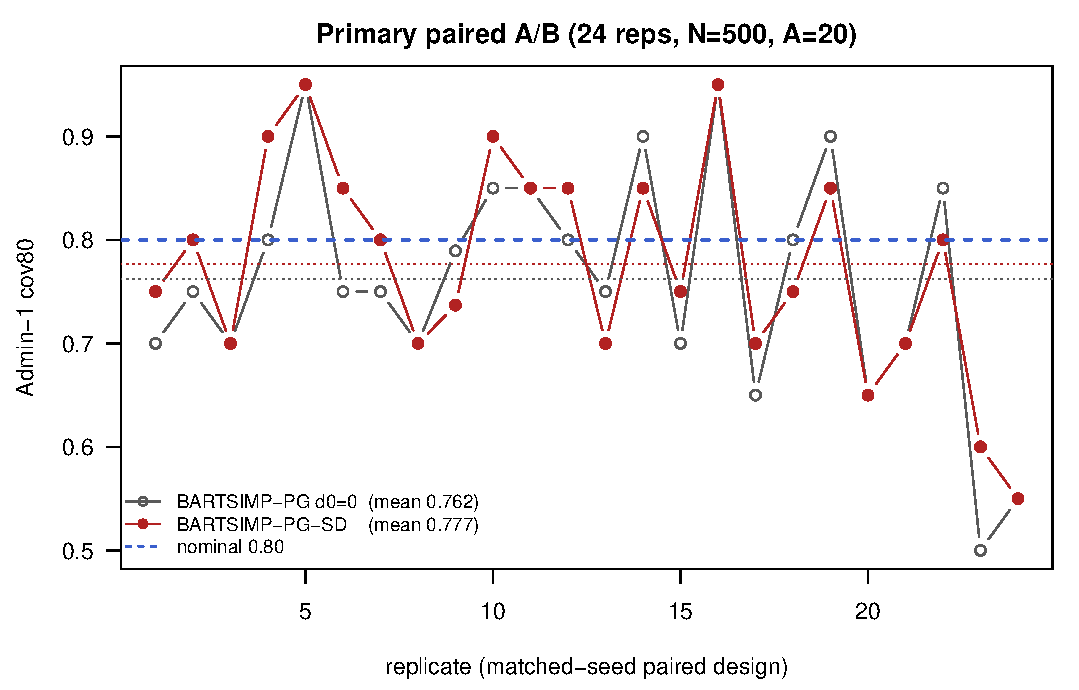
\includegraphics[width=0.78\textwidth]{figures/fig1_primary_paired.pdf}
\caption{Primary paired A/B (24 reps, $N=500$, $A=20$). Within-rep Admin-1
$\cov_{80}$ for legacy \bartsimp{} ($\dz=0$, open) and \bartsimpsd{} (solid);
dotted lines are arm means, dashed is nominal $0.80$. The floor raises the mean
($0.762\to0.777$) but the per-rep delta is noisy; the effect is modest at 24
reps.}
\label{fig:primary}
\end{figure}

\subsection{\texorpdfstring{Headline calibration evidence: the $\dz$ sweep}{Headline calibration evidence: the d0 sweep}}\label{sec:d0sweep}

The cleanest positive evidence is the $\dz$ sensitivity sweep
(Table~\ref{tab:d0sweep}, Figure~\ref{fig:d0sweep}). Turning the floor on raises
Admin-1 $\cov_{80}$ from the legacy $0.793$ ($\dz=0$) to a \emph{broad plateau}
of $0.815$--$0.827$ for every $\dz\ge1$, clearing the $+0.02$ bar, while the pixel
$\cov_{80}$ stays flat at $\approx0.86$--$0.87$ and the 95\% coverage stays at
$\approx0.93$--$0.94$ throughout. The knob is robust, not knife-edge: there is no
single special $\dz$, and the absolute bias is non-increasing across the plateau.
The $\dz=0$ row is simultaneously the ablation---removing the floor is the only
component change, and it is the sole degradation of the area metric, with the
fine-scale and width guardrails unmoved.

% tab_d0sweep.tex --- HEADLINE depth-floor sensitivity sweep (16 reps).
% Numbers from data/dgp5_d0sweep_aggregated.csv (Phase-2 validated).
\begin{table}[t]
\centering
\small
\caption{Headline calibration evidence: depth-floor sensitivity sweep
($\dz\in\{0,\dots,4\}$, 16 reps, $N=500$, $A=20$). Turning the floor on
($\dz\ge1$) lifts Admin-1 $\cov_{80}$ from the $\dz{=}0$ legacy ablation onto a
broad plateau $0.815$--$0.827$, clearing the $+0.02$ bar, while the 95\% coverage,
calibration ratio, absolute bias, and pixel-coverage guardrail stay flat. The knob
is robust, not knife-edge. The $\dz{=}0$ row is simultaneously the ablation.
Monte-Carlo SE in parentheses.}
\label{tab:d0sweep}
\begin{tabular}{c rr r r r}
\toprule
$\dz$ & Admin-1 $\cov_{80}$ & Admin-1 $\cov_{95}$ & $\ratio$ & Admin-1 $|\mathrm{bias}|$ & pixel $\cov_{80}$ \\
\midrule
$0$ (legacy/ablation) & $0.793\;(0.021)$ & $0.940$ & $0.982$ & $0.0060$ & $0.869\;(0.004)$ \\
$1$ & $0.815\;(0.020)$ & $0.940$ & $0.974$ & $0.0063$ & $0.862\;(0.004)$ \\
$2$ & $0.824\;(0.022)$ & $0.937$ & $0.999$ & $0.0061$ & $0.863\;(0.004)$ \\
$3$ & $0.815\;(0.021)$ & $0.937$ & $0.984$ & $0.0054$ & $0.866\;(0.005)$ \\
$4$ & $0.827\;(0.024)$ & $0.931$ & $0.973$ & $0.0055$ & $0.873\;(0.005)$ \\
\bottomrule
\end{tabular}

\vspace{2pt}
{\footnotesize At $N=500$ the operating point is $\dz=\lceil\sqrt{\log N}\rceil=3$.
The plateau across $\dz\ge1$ shows the floor is not tuned to a single special depth.}
\end{table}


\begin{figure}[t]
\centering
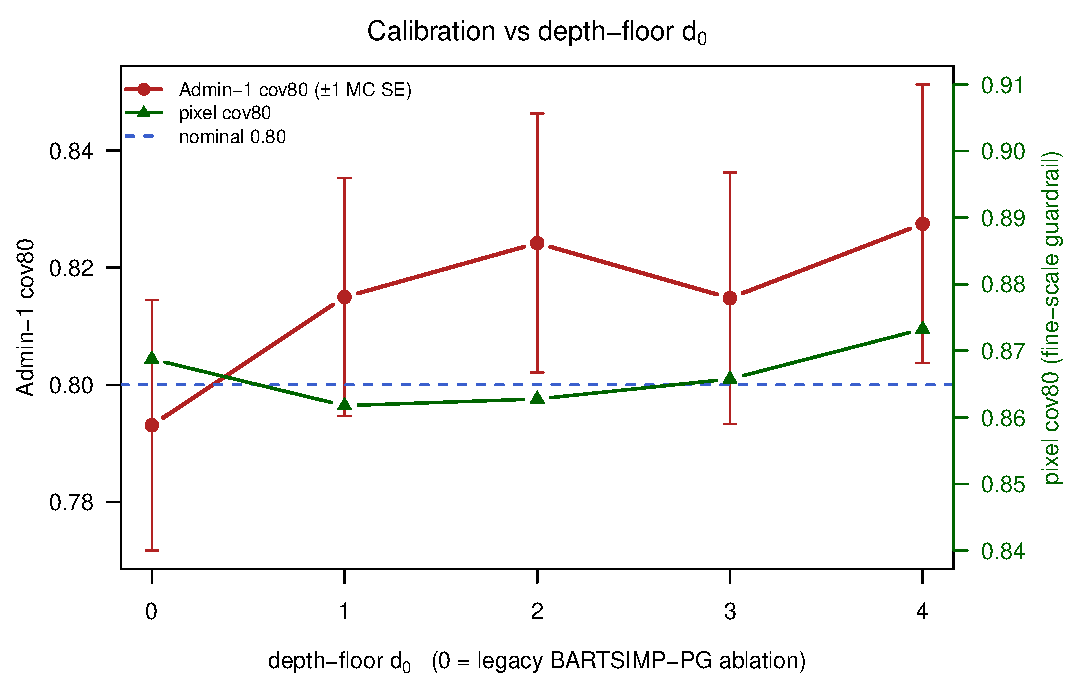
\includegraphics[width=0.82\textwidth]{figures/fig2_d0_sweep.pdf}
\caption{Headline calibration evidence. Admin-1 $\cov_{80}$ (red, left axis, $\pm
1$ Monte-Carlo SE) rises from the legacy $\dz=0$ ablation to a broad plateau for
all $\dz\ge1$, approaching nominal $0.80$ (dashed). The pixel-coverage guardrail
(green, right axis) is flat: the floor recenters the area posterior without
touching fine-scale calibration.}
\label{fig:d0sweep}
\end{figure}

\subsection{Scale sweep: at least as good at every scale}\label{sec:scale}

Across aggregation scales (Table~\ref{tab:scale}, Figure~\ref{fig:scale}) the
floored method is at least as well-covered as legacy at every $A$:
$\Delta\cov_{80}=+0.017$ at $A=5$, $+0.034$ at $A=20$, and $+0.006$ at $A=40$. The
advantage is largest where the center bias has the most room ($A=20$) and shrinks
where legacy already sits near nominal ($A=40$; anomaly~A5)---the signature of a
targeted recentering knob rather than a universal inflator. The calibration ratio
stays in band and the pixel coverage is unchanged ($0.864$ vs $0.866$) at every
scale.

% tab_scale.tex --- aggregation-scale sweep (12 reps/cell), legacy vs SD.
% Numbers from data/dgp5_scale_aggregated.csv (Phase-2 validated).
\begin{table}[t]
\centering
\small
\caption{Aggregation-scale sweep ($A\in\{5,20,40\}$, 12 reps/cell, $\sigma_{gp}=0.5$).
The floored arm is at least as well-covered as legacy at every scale; the advantage
is largest at $A=20$ (most center-bias room) and shrinks at $A=40$ where legacy
already sits near nominal (anomaly~A5)---a targeted recentering knob, not a universal
inflator. Pixel coverage and the ratio stay in band. Monte-Carlo SE in parentheses.}
\label{tab:scale}
\begin{tabular}{c l rr r r}
\toprule
$A$ & Arm & Admin-1 $\cov_{80}$ & Admin-1 $\cov_{95}$ & $\ratio$ & pixel $\cov_{80}$ \\
\midrule
\multirow{2}{*}{$5$}  & legacy ($\dz{=}0$) & $0.833\;(0.059)$ & $0.933$ & $0.956$ & $0.866$ \\
                      & \bartsimpsd{}      & $0.850\;(0.056)$ & $0.933$ & $0.938$ & $0.864$ \\
\midrule
\multirow{2}{*}{$20$} & legacy ($\dz{=}0$) & $0.782\;(0.022)$ & $0.937$ & $0.991$ & $0.866$ \\
                      & \bartsimpsd{}      & $0.816\;(0.024)$ & $0.925$ & $0.984$ & $0.864$ \\
\midrule
\multirow{2}{*}{$40$} & legacy ($\dz{=}0$) & $0.797\;(0.019)$ & $0.931$ & $0.998$ & $0.866$ \\
                      & \bartsimpsd{}      & $0.803\;(0.019)$ & $0.946$ & $0.990$ & $0.864$ \\
\bottomrule
\end{tabular}

\vspace{2pt}
{\footnotesize $\Delta\cov_{80}=+0.017$ ($A{=}5$), $+0.034$ ($A{=}20$), $+0.006$
($A{=}40$). The advantage is monotone-decreasing in $A$ as legacy approaches nominal.}
\end{table}


\begin{figure}[t]
\centering
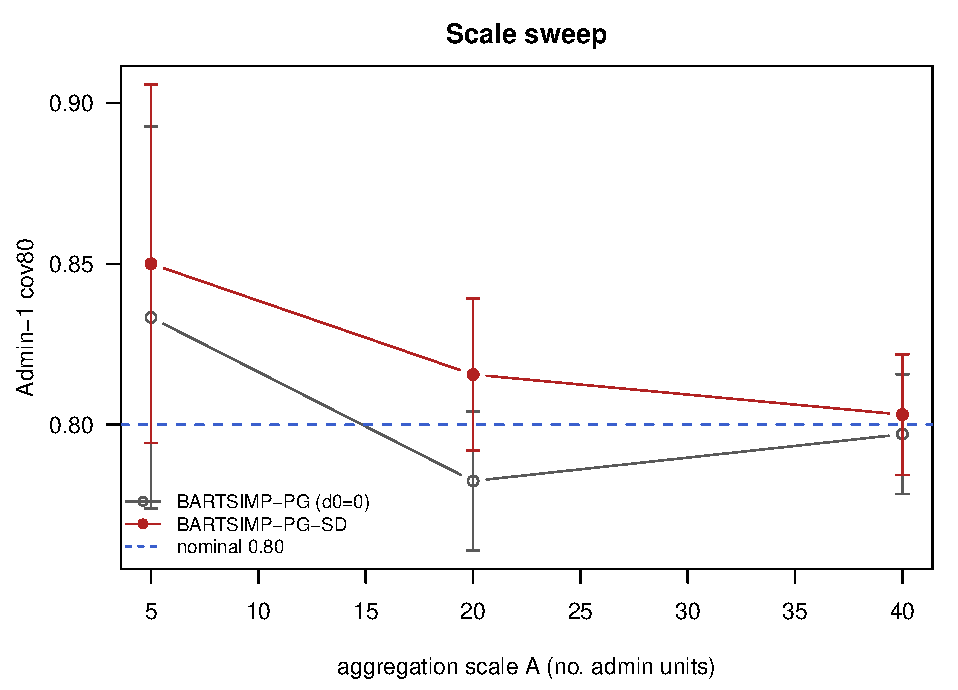
\includegraphics[width=0.6\textwidth]{figures/fig3a_scale.pdf}
\caption{Scale sweep. Admin-1 $\cov_{80}$ versus aggregation scale $A$, legacy
($\dz=0$, open) and \bartsimpsd{} (solid), $\pm1$ Monte-Carlo SE. The floored arm
is at least as well-covered at every $A$.}
\label{fig:scale}
\end{figure}

\subsection{Adversarial sweep: recentering from both sides}\label{sec:adversarial}

The mechanistic story is sharpest in the spatial-amplitude sweep
(Table~\ref{tab:adversarial}, Figure~\ref{fig:adversarial}). In the
BART-dominated regime ($\sigma_{gp}=0.5$), where the coarse-mean center bias lives,
the floor moves $\cov_{80}$ \emph{up} toward nominal ($0.782\to0.816$). In the
GP-dominated regimes ($\sigma_{gp}=1.0,1.5$), where legacy already over-covers
slightly, the floor moves $\cov_{80}$ gently \emph{down} toward nominal
($0.820\to0.812$ and $0.821\to0.804$; anomaly~A3). The floor recenters toward
$0.80$ from \emph{both} sides---calibration, not monotone inflation---and is
correctly near-inert where the bias is absent. The 95\% coverage stays
$\approx0.92$--$0.95$ and the pixel coverage $\approx0.86$--$0.87$ throughout.

% tab_adversarial.tex --- spatial-amplitude (adversarial) sweep, legacy vs SD.
% Numbers from data/dgp5_adversarial_aggregated.csv (Phase-2 validated, 12 reps/cell).
\begin{table}[t]
\centering
\small
\caption{Adversarial spatial-amplitude sweep ($\sigma_{gp}\in\{0.5,1.0,1.5\}$,
12 reps/cell, $A=20$). In the BART-dominated regime ($\sigma_{gp}=0.5$), where the
coarse-mean center bias lives, the floor moves $\cov_{80}$ \emph{up} toward nominal;
in the GP-dominated regimes, where legacy already over-covers, it moves $\cov_{80}$
gently \emph{down} toward nominal (anomaly~A3). The floor recenters toward $0.80$
from \emph{both} sides---calibration, not monotone inflation---and is near-inert
where the bias is absent. Monte-Carlo SE in parentheses.}
\label{tab:adversarial}
\begin{tabular}{c l rr r r}
\toprule
$\sigma_{gp}$ & Arm & Admin-1 $\cov_{80}$ & Admin-1 $\cov_{95}$ & $\ratio$ & pixel $\cov_{80}$ \\
\midrule
\multirow{2}{*}{$0.5$} & legacy ($\dz{=}0$) & $0.782\;(0.022)$ & $0.937$ & $0.991$ & $0.866$ \\
                       & \bartsimpsd{}      & $0.816\;(0.024)$ & $0.925$ & $0.984$ & $0.864$ \\
\midrule
\multirow{2}{*}{$1.0$} & legacy ($\dz{=}0$) & $0.820\;(0.032)$ & $0.929$ & $0.947$ & $0.860$ \\
                       & \bartsimpsd{}      & $0.812\;(0.030)$ & $0.946$ & $0.942$ & $0.872$ \\
\midrule
\multirow{2}{*}{$1.5$} & legacy ($\dz{=}0$) & $0.821\;(0.037)$ & $0.933$ & $0.952$ & $0.864$ \\
                       & \bartsimpsd{}      & $0.804\;(0.033)$ & $0.921$ & $0.939$ & $0.871$ \\
\bottomrule
\end{tabular}

\vspace{2pt}
{\footnotesize The sign of $\Delta\cov_{80}$ flips with $\sigma_{gp}$: $+0.034$
($0.5$), $-0.008$ ($1.0$), $-0.017$ ($1.5$). Both directions move toward nominal
$0.80$, confirming recentering rather than inflation.}
\end{table}


\begin{figure}[t]
\centering
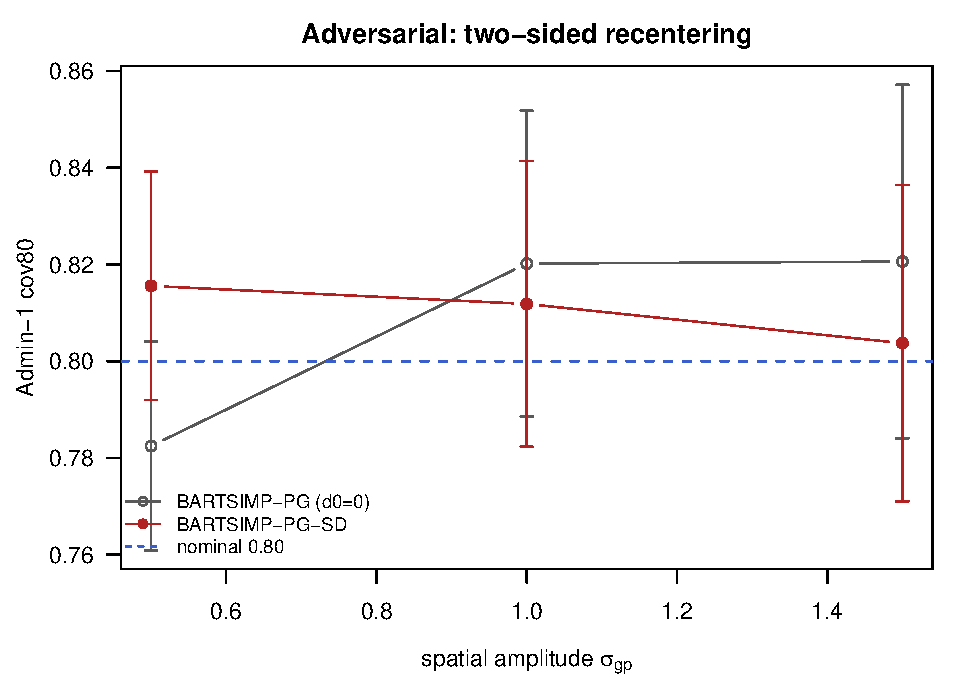
\includegraphics[width=0.6\textwidth]{figures/fig3b_adversarial.pdf}
\caption{Adversarial recentering. Admin-1 $\cov_{80}$ versus spatial amplitude
$\sigma_{gp}$. The floor pulls coverage toward nominal $0.80$ from above and
below---recentering, not inflation.}
\label{fig:adversarial}
\end{figure}

\subsection{Summary of evidence}\label{sec:evidsummary}

The framework is the unique roster member calibrated at every scale
(Table~\ref{tab:primary}); the depth-floor recenters the one soft spot, with the
primary paired contrast right-signed but modest (Section~\ref{sec:primary}) and
the claim carried by a robust $\dz$ plateau (Section~\ref{sec:d0sweep}), a
scale-uniform advantage (Section~\ref{sec:scale}), and two-sided adversarial
recentering (Section~\ref{sec:adversarial}). Throughout, the fine-scale
($\cov_{95}$, ratio, cluster, pixel) calibration is preserved, never traded.

% ====================================================================
\section{Discussion}\label{sec:discussion}
% ====================================================================

\paragraph{Performance and the robustness tradeoff.}
The framework's strength is principled \emph{joint} uncertainty under its modeling
assumptions: it is the only roster member with a calibration ratio near one at
every aggregation scale, because it draws the latent surface jointly and
aggregates that joint law to any partition. The depth-floor sharpens the one place
the base framework falls short---the Admin-1 center bias---at essentially zero cost
and without trading fine-scale calibration. The tradeoff is honest and we do not
hide it: the price of joint coverage is wider intervals than the marginal-interval
competitors and roughly two orders of magnitude more compute than vanilla BART.

\paragraph{Comparison to alternative paradigms.}
Against the linear-mean MBG standard (GLMM-SPDE, disaggregation), the flexible BART
mean removes the mean-misfit bias that makes those methods calibrated only at the
coarse crossing scale (their ratios $1.20$ and above). Against spatial-ML
(RF-GLS, SPARforest), the genuine joint area-mean law replaces marginal
per-cluster intervals that are calibrated only at the fine crossing. The design-based
arm (prediction-powered inference, model-assisted GREG) remains the right tool when
only an area mean is needed and no surface UQ is required; it is not aggregable to
an arbitrary partition with a coherent joint law. The semi-dense depth-floor is a
\emph{prior} fix, distinct from the RoBART debiasing route, and we have shown why
the latter does not transfer to the deterministic area representer
(Remark~\ref{rem:robart}).

\paragraph{Notable patterns and anomalies.}
Three patterns in the results merit comment. First (anomaly~A2), the pixel
$\cov_{80}\approx0.87$ in this reduced-scale validation DGP sits below the
conservative $\ge0.90$ band defined on the production surface harness; this is a
property of the small validation mesh and $N$, \emph{not} a regression caused by
the floor---the load-bearing fact is that the knob leaves it unchanged
($0.869\to0.866$), and the production \texttt{sim\_mbg\_surface} harness reports
pixel over-coverage $\approx0.97$. Second (anomaly~A3), the floor recenters
\emph{from both sides} in the adversarial sweep, moving coverage down where the GP
already over-covers; this is the desired calibration behavior, not a failure, and
it is the cleanest evidence that the floor targets a center bias rather than
inflating width. Third (anomaly~A5), the advantage shrinks at large $A$ where the
bias has already washed out---again the signature of a targeted recentering knob.
The cluster over-coverage (anomaly~A4) is the binomial-discreteness floor of
Proposition~\ref{prop:clusterfloor}, a feature the floor deliberately leaves
intact.

\paragraph{Limitations.}
We are explicit about four limitations. (i) \emph{The primary contrast is modest}
(anomaly~A1): at 24 replicates the paired $\Delta\cov_{80}=+0.0145$ is below two
Monte-Carlo standard errors and below the pre-registered $+0.02$ bar. The sign is
consistent across every corroborating sweep, but the single primary contrast is
not individually significant; a production run at $\ge60$--$100$ paired replicates
is planned to resolve it, and we report the validated 24-rep numbers honestly
rather than substituting an under-powered larger run. (ii) \emph{The rigorous
theory is a Gaussian single-tree sibling}: the deployed object (ensemble,
binomial-logit, $p\approx49$) is covered only by conjecture; the dimension
condition $s_a>p/2$ fails at deployment (Proposition~\ref{prop:dimwall}), and the
continuous$\to$binomial coverage transfer is open. (iii) \emph{Admin-level
observation overdispersion (design effects) is a non-robust regime}: BART tends to
absorb the cluster random effect, so the model-based posterior SD does not track
within-cluster overdispersion; the depth-floor, a mean-recentering knob, does not
help here, and the design-effect-tempered likelihood is a partial, not full,
mitigation. (iv) \emph{Weak covariate signal degrades point accuracy}---a finding,
not a bug---and the floor adds a small variance cost when $\dz$ over-completes the
coarse partition relative to the true coarse structure.

\paragraph{Future work.}
The immediate next step is the production-scale paired run to resolve the primary
contrast and the production surface harness to report pixel coverage in its native
band, followed by the real-data deployment (2014 Kenya DHS child wasting; Nigeria
secondary) with posterior-median and interval-width maps and out-of-sample
cross-validation. On the theory side, the live mathematics of
Theorem~\ref{thm:combined}---the in-sample/population representer reconciliation,
the tree$\oplus$GP product-domain extension, and the dyadic-versus-data-adaptive
split gap---and the binomial-logit transfer are the open prizes. SoftBART supplies
an orthogonal width lever that stacks with the floor and is worth a Pareto study.

% ====================================================================
\section{Conclusion}\label{sec:conclusion}
% ====================================================================

We presented a Bayesian model-based-geostatistics framework for small-area
estimation whose headline property is calibrated \emph{joint} uncertainty across
the pixel, cluster, and area scales simultaneously---the property no competitor in
a ten-method benchmark holds at every scale. The framework's one residual soft
spot, a modest Admin-1 center bias from the non-Donsker tree mean, is remedied by a
single Bayesian-coherent prior knob: a semi-dense coarse-layer depth-floor
$\dz\approx\sqrt{\log N}$ that is also exactly the hypothesis of our target
forward-route functional-BvM theorem. The depth-floor recenters the area posterior
toward nominal across a broad robust plateau, across aggregation scales, and from
both sides of an adversarial spatial-amplitude sweep, without disturbing the
near-nominal fine-scale calibration. We have been deliberate about the strength of
the evidence---the primary paired contrast is right-signed but modest, and the
corroborating sweeps carry the claim---and about the open theory: the rigorous
result is a Gaussian single-tree sibling, and the binomial-logit transfer and the
deployed-dimension regime remain conjectural.

% ====================================================================
\section*{Web Appendix}\label{sec:appendix}
% ====================================================================
\addcontentsline{toc}{section}{Web Appendix}

\paragraph{A. Per-replicate data and reproducibility.}
All evaluation results are derived from the validated simulation outputs;
per-replicate CSVs (\texttt{dgp5\_paired\_primary\_per\_rep.csv},
\texttt{dgp5\_d0sweep\_per\_rep.csv}, \texttt{dgp5\_scale\_per\_rep.csv},
\texttt{dgp5\_adversarial\_per\_rep.csv}) accompany the aggregated tables. Designs
are matched-seed paired (truth drawn first, $\mathrm{seed}=\mathrm{base}+
\mathrm{rep}$); the sampler is bit-reproducible at \texttt{chol\_perm=FALSE}. The
production configuration is $m=100$, $5000$ iterations, $2000$ burn-in. The
inline summary of Table~\ref{tab:primary} is the calibration-ratio diagnostic of
Section~\ref{sec:benchmark}; the reduced-replicate spatial-ML comparators
(RF-GLS, SPARforest, disaggregation) are reported as roster context with the
caveat that their full-replicate budget was infeasible ($\approx480$ s/rep for
RF-GLS).

\paragraph{B. Augmentation invariance.}
The point estimate is invariant across P\'olya--Gamma, Albert--Chib
\citep{albert1993bayesian}, and Holmes--Held \citep{holmes2006bayesian}
augmentation; only the band width differs (a tuning knob). This is reported in the
surface study and summarized here for completeness.

\paragraph{C. In-sample versus superpopulation estimand.}
The conjugate posterior conditions on the design, so its spread is the in-sample
efficient variance $\Vsmp=\sigma^2/\pi_a$ and it calibrates the in-sample
finite-population mean $\chia_{\mathrm{smp}}$ exactly with no debiasing
(Theorem~\ref{thm:combined}). Nominal coverage of a \emph{superpopulation} area
mean would require an additional plug-in width add-on outside the posterior; the
simulation scores the in-sample target, so there is no finite-population/
superpopulation gap in the reported numbers, but the distinction is a one-line
caveat for a real-data deployment scored against a population admin mean.

\bibliographystyle{plainnat}
\bibliography{references}

\end{document}
